\chapter{Datenstrukturen}
\label{appendix_datastructures}

\section{Übersicht über KMC-Operationen}
\label{dataops}

%% Übersicht über Operationen, die auf die zugrunde liegenden Datenstrukturen ausgeführt werden.
%% Zeitkritisch sind die unteren die Bereichs- und Oberflächensuche, da sie für jedes potentielle KMC-Ereignis ausgeführt werden müssen, die anderen nur für jedes versuchte.

\textbf{Konstruktion} \\
Der einmalige Aufbau aus einer Punktwolke.
Entspricht oftmals einer einzelnen Einfügung aller Punkte.
Die Laufzeit ist zweitrangig gegenüber den anderen Operationen
\\\\
\textbf{Einfügung} \\
Ergänzung eines Punktes zu einer bestehenden Struktur.
Wird nach erfolgten KMC-Ereignissen durchgeführt.
Laufzeiten: \BigO{1} (Listen) bis \BigO{n} (Nachbarschaftslisten)
\\\\
\textbf{Modifikation} \\
Aktualisierung der Position eines Punktes.
Entspricht gelegentlich einer Entfernung mit anschließender Einfügung.
Laufzeiten: \BigO{1} (Listen) bis \BigO{n} (Nachbarschaftslisten)
\\\\
\textbf{Entfernung} \\
Entfernung eines Punktes aus der Struktur, entspricht also oft einer inversen Einfügung.
Wird zur Entfernung von Oberflächen-Liganden aufgerufen.
Laufzeiten: wie bei der Einfügungs-Operation
\\\\
\textbf{Nachbarschaftssuche} \\
Extraktion einer Menge von Punkten in der Nähe anderer Punkte, z.B. für die Präparation von Ereignisse.
Geschieht für jeden Reaktionsversuch.
Laufzeiten: \BigO{1} (Nachbarschaftslisten) bis \BigO{n} (Listen)
\\\\
\textbf{Bereichssuche} \\
Extraktion einer Menge von Punkten in der Nähe eines beliebigen Punktes, z.B. zur Prüfung möglicher Reaktionen.
Wird für jede mögliche Reaktion durchgeführt und ist damit häufigste Operation.
Laufzeiten: \BigO{r_\text{s}^3} (Binning) bis \BigO{n} (Listen)
\\\\
\textbf{Oberflächensuche} \\
Die Bestimmung der globalen Oberfläche oder eines Punktes auf der Oberfläche entlang einer Geraden, je nach Prozess und verfügbaren Algorithmen.
Ist oft der limitierende Faktor der Simulation.
Delaunay-Triangulationen bilden per Alpha-Form implizit die globale Oberfläche ab, die so direkt in die KMC-Formulierung einfließen kann.


\section{Beschreibung grundlegender Datenstrukturen}
\label{appendix_dataoverview}

\begin{figure}[b]
  \captionsetup[subfigure]{singlelinecheck=false}{
    \def\subfigwidth{0.23\textwidth}
    \def\svgwidth{\textwidth}
    \begin{subfigure}[t]{\subfigwidth}
      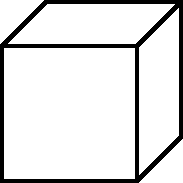
\includegraphics[width=\textwidth]{datastructures-a}
      \subcaption{Listen}
    \end{subfigure}
    \hfill
    \begin{subfigure}[t]{\subfigwidth}
      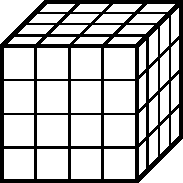
\includegraphics[width=\textwidth]{datastructures-b}
      \subcaption{Binning}
    \end{subfigure}
    \hfill
    \begin{subfigure}[t]{\subfigwidth}
      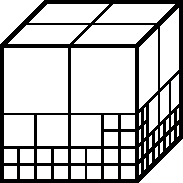
\includegraphics[width=\textwidth]{datastructures-c}
      \subcaption{Octree}
    \end{subfigure}
    \hfill
    \begin{subfigure}[t]{\subfigwidth}
      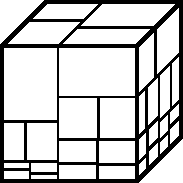
\includegraphics[width=\textwidth]{datastructures-d}
      \subcaption{k-d-Baum}
    \end{subfigure}
  }
  \caption[Übersicht über Partitionsmethoden des Simulationsraumes]{
    Übersicht über Partitionen des Simulationsraumes für einige Datenstrukturen.
    k-d-Baum-Partitionen sind dynamisch und ändern sich mit jeder Manipulation.
  }
  \label{fig:datastructures}
\end{figure}

\subsubsection{Atomlisten}

Die Atome des Simulationsraumes werden in einer unsortierten Liste gespeichert, ohne weitere Beziehungen zwischen den Atomen zu speichern.
Damit sind Manipulationsoperationen in konstanter Zeit \BigO{1} möglich, doch müssen Suchoperationen die gesamte Liste der Größe $n$ durchlaufen, wodurch sie für große Systeme durch Laufzeiten von \BigO{n} ungeeignet sind.

\subsubsection{Nachbarschaftslisten}

Nachbarschaftslisten speichern für jedes Atom eine Referenz auf die Atome in ihrer Nachbarschaft, wodurch Nachbarschaftssuchen effizienter werden, aber jede Manipulation eine Aktualisierung der Nachbarschafts-Referenzen jedes Atomes verursachen.
Die anderen Suchoperationen haben von den Referenzen keine Vorteile und behalten deshalb die Laufzeit von \BigO{n} gegenüber den Atomlisten.
Für MD-Simulationen lohnen sich Nachbarschaftslisten jedoch, da sich die Nachbarschaft nur langsam ändert, aber die meisten Kraftfelder auf eine feste Reichweite begrenzt sind, wodurch mit NB-Listen nur die Kräfte über relevante Atome untersucht werden.

\subsubsection{Binning-Methoden}
Beim Binning werden Punkte in meist quaderförmige Raumbereiche (Bins) eingeteilt, wodurch bei Suchoperationen vom Zustand der Bins Rückschlüsse auf das Suchergebnis gezogen werden können.
Die Koordinaten des Bins ergibt sich aus der globalen Position der Atome durch lineare Beziehungen.
Innerhalb der Bins liegen wiederum Atomlisten vor, doch werden die Maße der Bins oberhalb der Manipulations-Reichweiten gewählt, sodass die Nachteile der Atomlisten unterdrückt werden.
Bins selbst können in einer übergeordneten Datenstruktur verwaltet werden, beispielsweise die in Abschnitt~\ref{dataoctree} verwendeten Octrees.

\subsubsection{Suchbäume}
In Suchbäumen wird jedes Atom entsprechend seiner Position als Knoten eines balancierten Binär-Baumes verwaltet, sodass Suchoperationen in \BigO{\log{n}} terminieren.
Durch seine Formulierung müssen die Beziehungen zwischen den Knoten rekursiv aktualisiert werden, wofür gelegentlich der gesamte Baum aufwendig umstrukturiert werden muss.
Eine mögliche Form wird mit dem k-d-Baum in Abschnitt~\ref{datakdtree} vorgestellt.

\subsubsection{Triangulationen}
Triangulationen zerlegen den Simulationsraum raumfüllend in $k$-Simplexe\footnote{Ein $k$-Simplex ist ein Objekt in $k$ Dimensionen mit $k+1$ Eckpunkten, die untereinander mit geraden Kanten verbunden sind.
  Somit ist ein 1-Simplex eine Linie, ein 2-Simplex ein Dreieck, ein 3-Simplex ein Tetraeder, usw.}, an deren Eckpunkten sich die Atome befinden.
Je nach Konstruktionskriterium werden dadurch implizit einige Eigenschaften der Punktwolke dargestellt.
Abschnitt~\ref{datadelaunay} stellt Delaunay-Triangulationen vor, welche durch Beschreibung der Oberfläche der Punktwolke und der Nächstnachbarbeziehungen der Atome schnelle Oberflächen- und Nachbarschaftssuchen auf Kosten der Konstruktion ermöglichen, im Gegensatz zu Suchbäumen aber partitionierbar sind.

\section{Delaunay-Triangulationen}
\label{appendix_delaunay}

\subsection{Ausgewählte Eigenschaften einer Delaunay-Triangulation}

\begin{itemize}
\item Jeder Punkt ist Eckpunkt eines oder mehrerer Simplexe
\item Simplexe überschneiden sich nicht
\item Im Umkreis eines Simplexes befinden sich keine weiteren Punkte
\item Die Vereinigung aller Simplexe ergibt die konvexe Hülle
\item Alpha-Form $\subset$ Delaunay-Triangulation
\item %Ein Punkt teilt sich mit seinem nächsten Nachbarn mindestens einen Simplex \\
  %$\Leftrightarrow$
  Nächstnachbargraph $\subset$ Delaunay-Triangulation
  %% \item Die Delaunay-Triangulation und das Voronoi-Diagramm über die selben Punkte sind dual\\
  %% $\Rightarrow$ Allgemeine Nachbarschaftssuche ist \BigO{k\log k}
\end{itemize}

\subsection{Algorithmen zur Konstruktion einer Delaunay-Triangulation}

Zur Delaunay-Triangulierung aus einer Punktmenge stehen verschiedene Algorithmen zur Verfügung, die auf unterschiedlichen Methoden aufbauen.
\\\\
\textbf{Flip-basierte Algorithmen (Local Improvement)}\\
Der Algorithmus startet mit einer beliebigen Triangulation, prüft den Umkreis aller Simplexe auf enthaltene Punkte und korrigiert gegebenenfalls per Flip-Algorithmus, der in Abbildung~\ref{fig:delaunay-flip} dargestellt ist.
Diese Algorithmen konvergieren typischerweise in \BigO{n^2} und sind damit vergleichsweise langsam.
\\\\
\textbf{Scan-Algorithmus (Incremental Construction)}\\
Der Algorithmus konstruiert schrittweise Simplexe, die das Delaunay-Kriterium erfüllen und keine nachträgliche Änderung benötigen.
Durch viele Vergleiche und Sortierungen variieren typische asymptotische Laufzeiten zwischen \BigO{n\log{n}} und \BigO{n^2}.
\\\\
\textbf{Einfügungs-Algorithmen (Incremental Insertion)}\\
Der Algorithmus erstellt einen beliebig großen Simplex, der die gesamte Punktmenge beinhaltet, und fügt schrittweise einzelne Punkte in die Triangulation ein.
Der den eingefügten Punkt umfassende Simplex wird an diesem Punkt in mehrere Unter-Simplexe geteilt, auf die und deren unmittelbare Nachbarn ein Flip-basierter Algorithmus ausgeführt wird.
Laufzeiten sind typischerweise gering mit \BigO{n\log{n} + n^{\lceil d/2 \rceil}}.
\\\\
\textbf{Divide-and-Conquer-Algorithmen}\\
Der Algorithmus teilt die Punktmenge in Untermengen, die rekursiv trianguliert und anschließend an ihren Grenzen miteinander kostspielig zur Zieltriangulation vereinigt werden, wodurch er parallelisierbar ist.
%% Größter Rechenaufwand ist für die Vereinigung der Teiltriangulierungen notwendig, die in höheren Dimensionen nicht-trivial ist.
Mit dem DeWall-Algorithmus\cite{cignoni_dewall:_1998} ist eine Laufzeit von \BigO{n^{\lceil d/2 \rceil + 1}} m;glich, wobei der Vereinigungs-Algorithmus auch für die Einfügung von Blöcken in bestehende Strukturen sowie für teilperiodische Räume interessant ist.
\\\\
\textbf{Höherdimensionale Einbettung}\\
Hier wird die Punktmenge in eine höhere Dimension transformiert, in der deren konvexe Hülle berechnet wird, die dann in den ursprünglichen Raum herunter projiziert wird und darin eine gültige Delaunay-Triangulation ergibt.
Dieser Algorithmus ist von rein akademischem Interesse, wird aber ebenfalls bei Hinzufügung und Aktualisierung von Punkten interessant.

\begin{figure}[b]
  \captionsetup[subfigure]{singlelinecheck=false}{
    \def\subfigwidth{0.23\textwidth}
    \def\svgwidth{\textwidth}
    \begin{subfigure}[t]{\subfigwidth}
      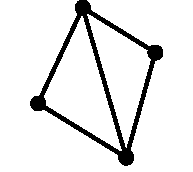
\includegraphics[width=\textwidth]{delaunay-flip-a}
      \subcaption{Ausgangstriangulation}
      \label{fig:delaunay-flip-a}
    \end{subfigure}
    \hfill
    \begin{subfigure}[t]{\subfigwidth}
      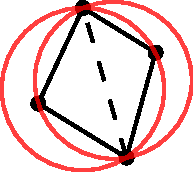
\includegraphics[width=\textwidth]{delaunay-flip-b}
      \subcaption{Vereinigung invalider Simplexe}
      \label{fig:delaunay-flip-b}
    \end{subfigure}
    \hfill
    \begin{subfigure}[t]{\subfigwidth}
      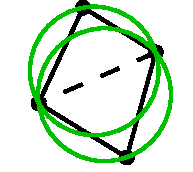
\includegraphics[width=\textwidth]{delaunay-flip-c}
      \subcaption{Aufteilung in neue valide Simplexe}
      \label{fig:delaunay-flip-c}
    \end{subfigure}
    \hfill
    \begin{subfigure}[t]{\subfigwidth}
      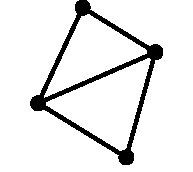
\includegraphics[width=\textwidth]{delaunay-flip-d}
      \subcaption{Ergebnis}
      \label{fig:delaunay-flip-d}
    \end{subfigure}
  }
  \caption[Flip-Algorithmus für Delaunay-Triangulationen]{
    Flip-Algorithmus: Invalide Simplexe werden aufgelöst und entlang einer neuen Kontaktfläche in valide Simplexe überführt.
    Anschließend müssen die Nachbarn auf das Delaunay-Kriterium geprüft und gegebenenfalls geflippt werden.
    %% Diese Operation läuft in \BigO{k_d\log{k_d}} Prüfungen bei Aktualisierung der Punkte eines Simplexes, mit $k_d$ als oberer Schranke der Zahl der Simplexe eines Punktes.
  }
  \label{fig:delaunay-flip}
\end{figure}
